\section{Auswertung}
\label{sec:Auswertung}

\subsection{Untergrund}
\label{sec:Unter}
Für die Bestimmung des Untergrunds von $j(T)$ werden die Messdaten außerhalb von \SI{230}{\kelvin} bis \SI{280}{\kelvin} herangezogen.
Diese sind in den Abbildungen \ref{fig:plot1} und \ref{fig:plot2} blau dargestellt.
Des Weiteren ist auch der Untergrundfit der Form
\begin{equation}
    \label{eqn:exp}
    I(T) = a \cdot T + b
\end{equation}
in den Abbildungen \ref{fig:plot1} und \ref{fig:plot2} eingezeichnet.
Aufgrund des abflachenden Anstiegs nach \SI{280}{\kelvin} ist es nicht möglich eine Expontentialfunktion als Fitfunktion zu verwenden.
Die Parameter für die Heizrate 1 von etwa \SI{1.43(28)}{\kelvin\per\minute} ergeben sich zu
\begin{align*}
    a_1 &= \SI{0.070(2)e-12}{\ampere\per\kelvin} \\
    b_1 &= \SI{-15.1(6)e-12}{\ampere}.
\end{align*}
und für die Heizrate 2 von etwa \SI{1.91(22)}{\kelvin\per\minute} zu
\begin{align*}
  a_2 &= \SI{0.100(3)e-12}{\ampere\per\kelvin} \\
  b_2 &= \SI{-21.9(8)e-12}{\ampere}.
\end{align*}
Die Heizraten werden aus dem Mittelwert der mittleren Änderungsraten zwischen zwei Datenpunkten bestimmt.
Nach der Subtraktion des Untergrunds, sind einige Messwerte kleiner als Null.
Die bereinigten Daten werden um diesen Offset (in den Abbildungen \ref{fig:plot1} und \ref{fig:plot2} gelb) korrigiert.

\begin{figure}
  \centering
  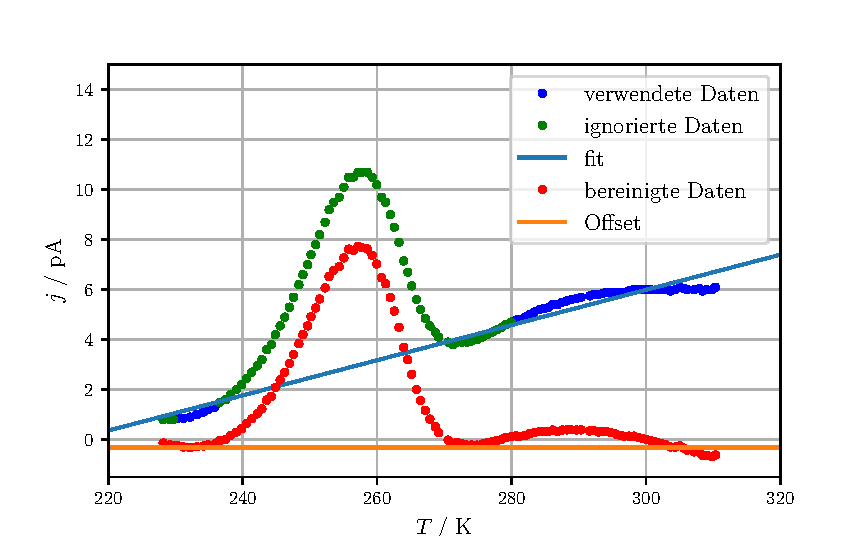
\includegraphics{plot1.pdf}
  \caption{Depolaristaionsstrom und Temperatur für die Heizrate \SI{1.43}{\kelvin\per\minute}. Nicht verwendete Messdaten sind grün und die für den Untergrund verwendeten blau. Die bereinigten Daten sind rot, der Offset gelb.}
  \label{fig:plot1}
\end{figure}
\begin{figure}
  \centering
  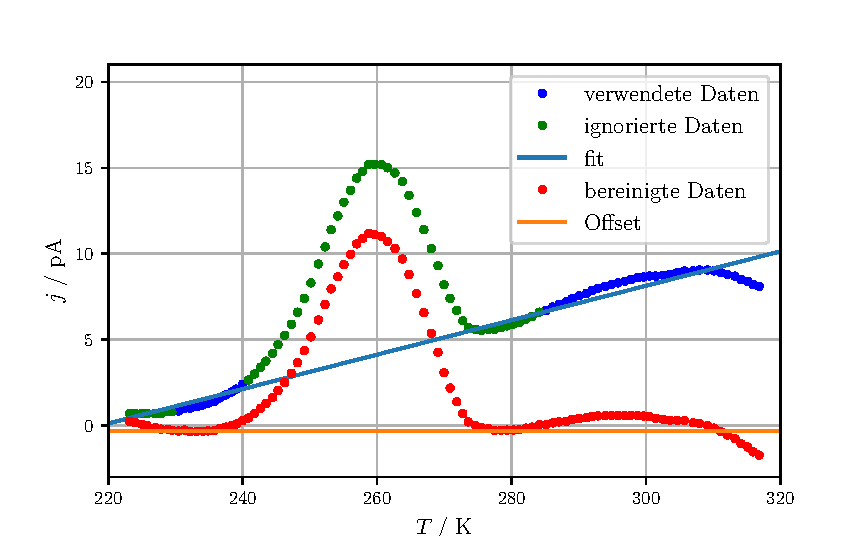
\includegraphics{plot2.pdf}
  \caption{Depolaristaionsstrom und Temperatur für die Heizrate \SI{1.91}{\kelvin\per\minute}. Nicht verwendete Messdaten sind grün und die für den Untergrund verwendeten blau. Die bereinigten Daten sind rot, der Offset gelb.}
  \label{fig:plot2}
\end{figure}

\subsection{Stromdichteansatz}
\label{sec:klT}
Zur Berechnung der Aktivierungsenergie $W$ bei kleinen Temperaturen werden die Daten im Bereich von \SI{236}{\kelvin} bis \SI{255}{\kelvin} für die erste Messung verwendet, für die zweite Messung im Bereich von \SI{236}{\kelvin} bis \SI{255}{\kelvin}.
Diese Bereiche sind in der halblogarithmischen Darstellung annähernd linear.
Es wird die Näherung der Stromdichte für kleine Temperaturen herangezogen.
Der gemessene Strom $i(T)$ ist dabei bis auf einen konstanten Faktor proportional zur Stromdichte.
Der Strom wird logarithmiert und in Abhängigkeit von der reziproken Temperatur $\frac{1}{T}$ aufgetragen.
Für jede Heizrate erfolgt eine lineare Ausgleichsrechnung der Form
\begin{equation}
    \label{eqn:lin}
    \ln\left(\frac{i(T)}{\SI{1e-11}{\ampere}}\right) = -\frac{W}{\symup{k_B} T} + c,
\end{equation}
welche in Abbildung \ref{fig:plot3} für Heizrate 1 und in Abbildung \ref{fig:plot3} für Heizrate 2 abgebildet sind.
Somit lassen sich die Aktivierungsenergien $W_\text{i} = -a_\text{i} \cdot \symup{k_B}$ und die Konstanten zu
\begin{align*}
    W_1 &= \SI{0.95(4)}{\electronvolt} \\
    W_2 &= \SI{1.15(5)}{\electronvolt} \\
    c_1 &= \num{18.0(18)} \\
    c_2 &= \num{27.4(22)}
\end{align*}
bestimmen.

\begin{figure}
  \centering
  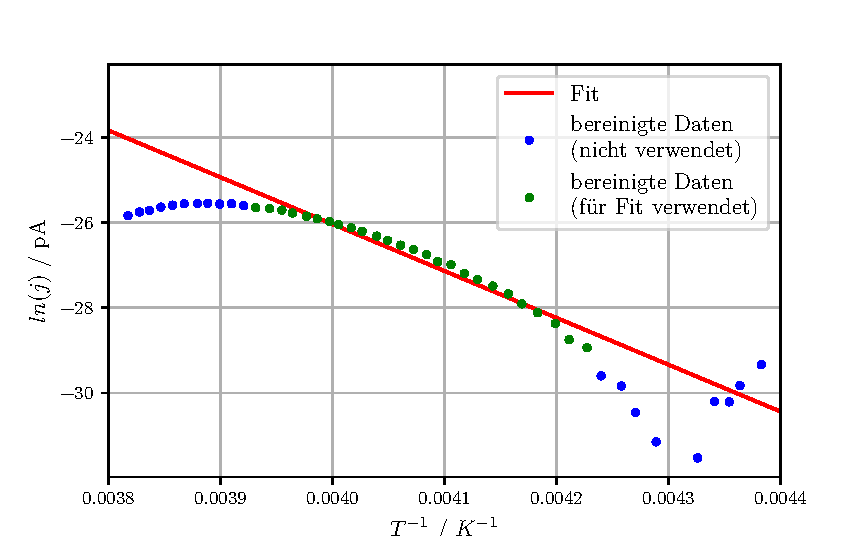
\includegraphics{plot3.pdf}
  \caption{Halblogarithmische Darstellung des Stroms in Abhängigkeit der reziproken Temperatur bei kleinen Temperaturen für den Stromdichteansatz bei der Heizrate \SI{1.43}{\kelvin\per\minute} und die dazugehörige Ausgleichsgerade.}
  \label{fig:plot3}
\end{figure}
\begin{figure}
  \centering
  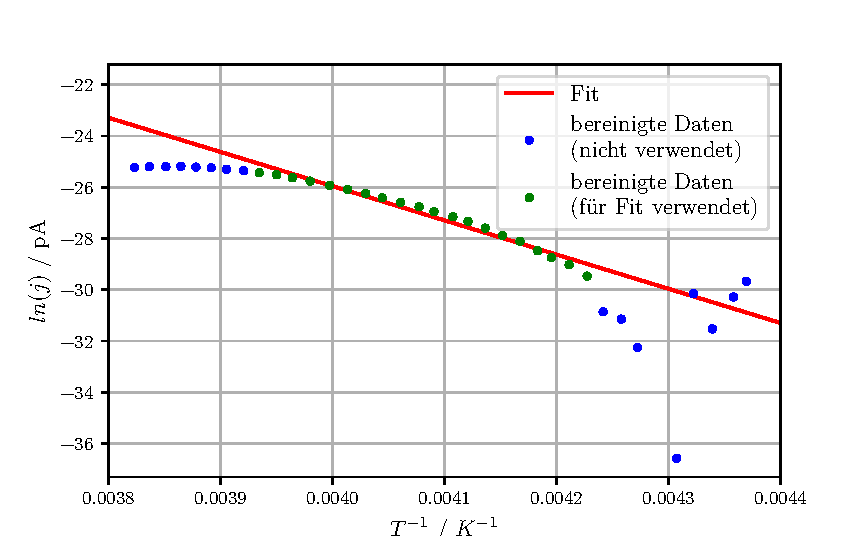
\includegraphics{plot4.pdf}
  \caption{Halblogarithmische Darstellung des Stroms in Abhängigkeit der reziproken Temperatur bei kleinen Temperaturen für den Stromdichteansatz bei der Heizrate \SI{1.91}{\kelvin\per\minute} und die dazugehörige Ausgleichsgerade.}
  \label{fig:plot4}
\end{figure}

\subsection{Polarisationsansatz}
\label{sec:grT}
Nun wird die Aktivierungsenergie auf Grundlage des Polarisationsansatzes bestimmt.
Hierzu werden die Daten im Bereich von \SI{240}{\kelvin} bis \SI{265}{\kelvin} für die erste Messung verwendet, für die zweite Messung im Bereich von \SI{240}{\kelvin} bis \SI{276}{\kelvin}.
Dazu wird eine numerische Integration der Form
\begin{equation}
    \label{eqn:int}
    \int_T^{T^*} i(T') \symup{d}\,T'
\end{equation}
durchgeführt.
Dies erfolgt mit \textit{Scientific Python} \cite{scipy} und der Trapez-Regel.
Dabei ist zu beachten, dass $j(T^*) \approx \SI{0}{\ampere}$ gelten muss.
Dies lässt sich für die Heizrate 1 auf $T^*_1 = \SI{275.85}{\kelvin}$ und für die Heizrate 2 auf $T^*_2 = \SI{278.45}{\kelvin}$ approximieren, da diese den kleinsten absoluten Abstand zu \SI{0}{\ampere} haben.
Wird nun
\begin{equation*}
    \ln\left(\frac{\int_T^{T^*} i(T') \symup{d}\,T'}{b_i \cdot i(T)}\right)
\end{equation*}
gegen $\frac{1}{T}$ aufgetragen und eine lineare Ausgleichrechnung der Form
\begin{equation}
    \label{eqn:lin2}
    \ln\left(\frac{\int_T^{T^*} i(T') \symup{d}\,T'}{b_i \cdot i(T)}\right) = \frac{W}{\symup{k_B} \cdot T} + \ln(\tau_0) = \frac{W}{\symup{k_B} \cdot T} + d
\end{equation}
durchgeführt, lässt sich die Aktivierungsenergie und theoretisch aus dem Parameter $d$ die Relaxationszeit $\tau_0$ bestimmen, was hier auf Grund des unbekannten Offsets nicht möglich ist.
Die in Abbildung \ref{fig:plot5} gezeigte Ausgleichsgerade für Heizrate 1 ergibt die Parameter
\begin{align*}
    W_1 &= \SI{1.114(33)}{\electronvolt} \\
    d_1 &= \num{-48.8(15)}
\end{align*}
Für die Heizrate 2 (siehe Abbildung \ref{fig:plot6}) ergeben sich diese Werte zu
\begin{align*}
    W_2 &= \SI{0.985(14)}{\electronvolt} \\
    d_2 &= \num{-42.1(6)}.
\end{align*}

\begin{figure}
  \centering
  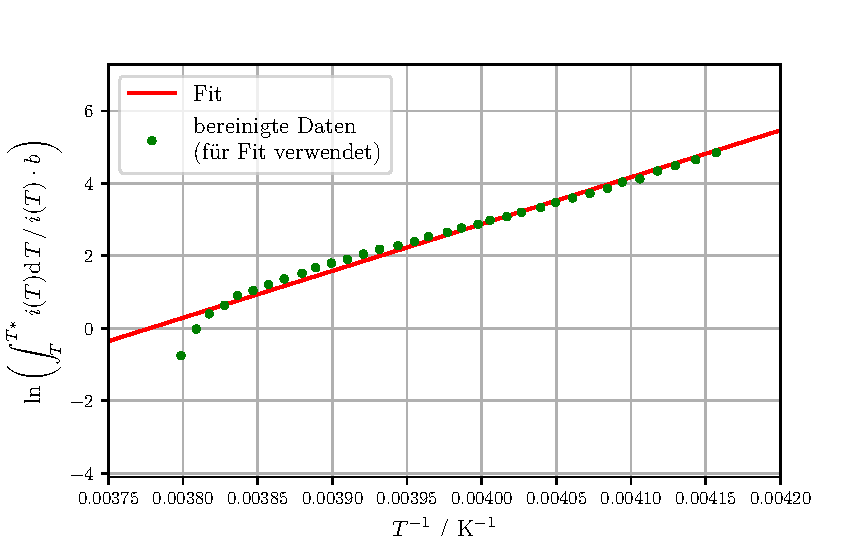
\includegraphics{plot5.pdf}
  \caption{Reziproke Temperatur und integrierter Strom zur Bestimmung der Aktivierungsenergie nach dem Polarisationsansatz für die Heizrate \SI{1.43}{\kelvin\per\minute}.}
  \label{fig:plot5}
\end{figure}
\begin{figure}
  \centering
  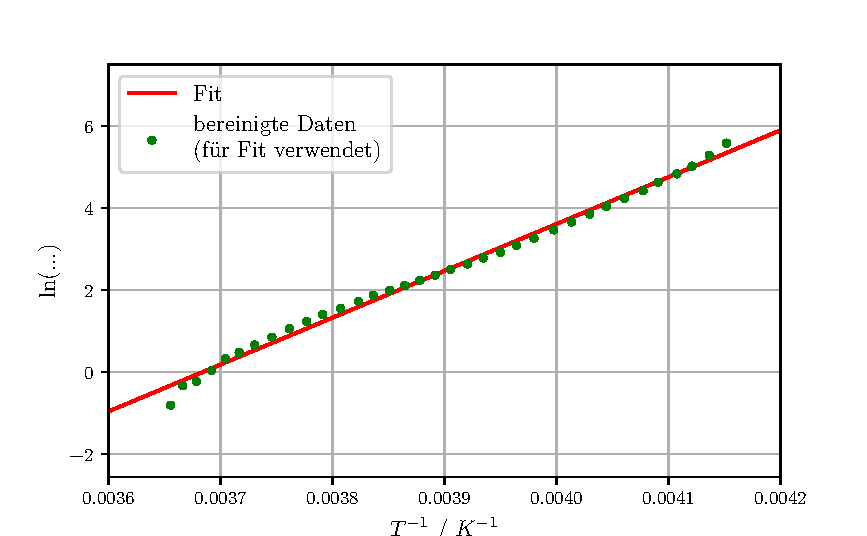
\includegraphics{plot6.pdf}
  \caption{Reziproke Temperatur und integrierter Strom zur Bestimmung der Aktivierungsenergie nach dem Polarisationsansatz für die Heizrate \SI{1.91}{\kelvin\per\minute}.}
  \label{fig:plot6}
\end{figure}
\FloatBarrier

\subsection{Relaxationszeit}
\label{sec:relax}
Des Weiteren lässt sich aus dem Maximum von $j(T)$ auch die charakteristische Relaxationszeit $\tau_0$
bestimmen:
\begin{equation}
    \label{eqn:tau0}
    \tau_0 = \frac{\symup{k_B}T_\text{max}^2}{W \cdot b} \exp\left(-\frac{W}{\symup{k_B}T_\text{max}} \right).
\end{equation}
Der Fehler ergibt sich dabei nach
\begin{align*}
    \label{eqn:FehlerTau}
    \Delta \tau_0 & =\sqrt{\left(\frac{\symup{k_B} T_\text{max}^2}{W \cdot b} \exp\left(-\frac{W}{\symup{k_B} T_\text{max}}\right)\left(-\frac{1}{\symup{k_B}T_\text{max}} - \frac{1}{W} \right) \Delta W \right)^2} \\
    &\overline{+ \left(-\frac{\symup{k_B} T_\text{max}^2}{W \cdot b^2} \exp\left(-\frac{W}{\symup{k_B} T_\text{max}}\right)\Delta b \right)^2}.
\end{align*}
Dabei wird für $T_\text{max}$ das Maximum der jeweiligen Heizrate nach Abzug des Untergrunds bestimmt.
Die Heizraten werden aus dem Mittelwert der mittleren Änderungsraten zwischen zwei Datenpunkten bestimmt.
Wie bereits erwähnt ist eine Heizrate \SI{1.43(28)}{\kelvin\per\minute} und die andere Heizrate \SI{1.91(22)}{\kelvin\per\minute}.
Die Relaxationszeit wird für alle vier berechneten Aktivierungsenergien einzeln bestimmt.
\begin{align*}
  \tau_0(\text{Heizrate 1, Stromdichte}) &= \SI{1.1(19)e-18}{\second} \\
  \tau_0(\text{Heizrate 1, Polarisation}) &= \SI{5(8)e-22}{\second} \\
  \tau_0(\text{Heizrate 2, Stromdichte}) &= \SI{1.1(23)e-22}{\second} \\
  \tau_0(\text{Heizrate 2, Polarisation}) &= \SI{2.0(13)e-19}{\second} \\
\end{align*}
%Der Fehler ergibt sich dabei nach
%\begin{align*}
%    \label{eqn:FehlerTau}
%    \Delta \tau_0 & = \sqrt{\left(\frac{\symup{k_B}}{W h} \exp\left(-\frac{W}{\symup{k_B} T_\text{max}}\right) \left(\frac{W}{\symup{k_B}} + 2 T_\text{max}\right) \Delta T_\text{max} \right)^2} \\
%    &\overline{+ \left(\frac{\symup{k_B} T_\text{max}^2}{h} \exp\left(-\frac{W}{\symup{k_B} T_\text{max}}\right)\left(\frac{W}{\symup{k_B}T_\text{max}} + 1 \right) \Delta W \right)^2} \\
%    &\overline{+ \left(\frac{\symup{k_B} T_\text{max}^2}{h} \exp\left(-\frac{W}{\symup{k_B} T_\text{max}}\right)\Delta b \right)^2}.
%\end{align*}
%Zu beachten ist, dass kein Fehler für $T_\text{max}$ angenommen wurde, womit der Teil mit $\Delta T_\text{max}$ in der Gauß'schen Fehlerfortpflanzung enfällt.
